\documentclass[a4paper]{jpconf}

\usepackage{graphicx}
%\usepackage{units}
%%%%%%%%%%%%%%%%%%%%%%%%%%
%\usepackage[dvips]{graphicx}            % to include images
	%\usepackage{jpeg2pslatex}
%\restylefloat{figure}
%\usepackage{float}
%\usepackage{amsmath}
\usepackage{array}
\usepackage{subcaption}
\DeclareGraphicsExtensions{.png,.pdf}

%%%%%%%%%%%%%%%%%%%%
\usepackage{amssymb}
% some new commands
\newcommand{\diffD}{\ensuremath{\mathcal{D}}}
\newcommand{\Z}{\ensuremath{Z}}
\newcommand{\Higgs}{\ensuremath{H}}
\newcommand{\Zp}{\ensuremath{Z_d}}
\newcommand{\HZpZp}{\ensuremath{H \rightarrow \Zp\Zp}}
\newcommand{\HZpZpllll}{\ensuremath{\HZpZp \rightarrow \llll}}
\newcommand{\HZZ}{\ensuremath{H \rightarrow \Z\Z^{*}}}
\newcommand{\HZZllll}{\ensuremath{\HZZ \rightarrow \llll}}
\newcommand{\HZZp}{\ensuremath{H \rightarrow \Z\Zp}}
\newcommand{\HZZpllll}{\ensuremath{\HZZp \rightarrow \llll}}
\newcommand{\Zpll}{\ensuremath{\Zp \rightarrow \ell^+\ell^-}}
\newcommand{\Zll}{\ensuremath{\Z \rightarrow \ell^+\ell^-}}
\newcommand{\llll}{\ensuremath{4\ell}}
\newcommand{\ZZllll}{\ensuremath{ZZ^{*} \rightarrow 4\ell}}
\newcommand{\ZZeeee}{\ensuremath{ZZ^{*} \rightarrow 4e}}
\newcommand{\ZZeemm}{\ensuremath{ZZ^{*} \rightarrow 2e2\mu}}
\newcommand{\ZZmmmm}{\ensuremath{ZZ^{*} \rightarrow 4\mu}}
\newcommand{\Wetal}{Wells \textit{et al}}
\newcommand{\MeV}{\ensuremath{\mbox{MeV}}}
\newcommand{\GeV}{\ensuremath{\mbox{GeV}}}
\newcommand{\TeV}{\ensuremath{\mbox{TeV}}}
\newcommand{\PhiSM}{\ensuremath{\Phi_{\text{\tiny{SM}}}}}
\newcommand{\mPhiSM}{\ensuremath{m_{\Phi_{\text{\tiny{SM}}}}}}
\newcommand{\sigmaHAHM}{\ensuremath{\sigma_{\text{\tiny{HAHM}}}}}
\newcommand{\sigmaSM}{\ensuremath{\sigma_{\text{\tiny{SM}}}}}
\newcommand{\BRHAHM}{\ensuremath{\text{BR}_{\text{\tiny{HAHM}}}}}
\newcommand{\BRSM}{\ensuremath{\text{BR}_{\text{\tiny{SM}}}}}
\newcommand{\ifb}{fb\textsuperscript{-1}}
\newcommand{\thetaMC}{\ensuremath{\theta_{\text{\tiny{MC}}}}}
\newcommand{\Haa}{\ensuremath{H \rightarrow aa}}
\newcommand{\Haallll}{\ensuremath{\Haa \rightarrow 4\mu}}
\newcommand{\bbbarbbbar}{\ensuremath{b\bar{b}b\bar{b}}}
\newcommand{\qqbar}{\ensuremath{q\bar{q}}}
\def\progname#1{{\textsc{ #1}}}
\newcommand*{\hfourl}{\ensuremath{H \rightarrow ZZ^* \rightarrow 4\ell}}
\newcommand*{\hzdfourl}{\ensuremath{H \rightarrow ZZ_d \rightarrow 4\ell}}
\newcommand*{\zjets}{\ensuremath{Z+\mathrm{jets}}}
\newcommand*{\ttV}{\ensuremath{t\bar{t}V}}
\newcommand*{\ttZ}{\ensuremath{t\bar{t}Z}}
\newcommand*{\ttW}{\ensuremath{t\bar{t}W}}
\newcommand*{\ttH}{\ensuremath{t\bar{t}H}}
\newcommand*{\bbH}{\ensuremath{b\bar{b}H}}
\newcommand{\zzstar}{\ensuremath{ZZ^{*}}}
\newcommand{\llee}{\ensuremath{\ell\ell ee}}
\newcommand{\llmumu}{\ensuremath{\ell\ell \mu\mu}}
%\newcommand*{\ttZ}{\ensuremath{t\bar{t}+Z}}


\begin{document}
\title{Fluid flow and humidity in the ATLAS ITk studied by CFD}

\small{
\author{M Bhamjee$^{1}$, P Mafa$^{2}$, L Leeuw$^{2}$, SH Connell$^1$}

\address {
1. University of Johannesburg, Johannesburg, Mechanical Engineering, South Africa.\\
2. University of South Africa, Johannesburg, Physics, South Africa
}}
\normalsize

\ead{muaazb@uj.ac.za}
\vspace{-10pt}
\begin{abstract}
CERN has planned a series of upgrades for the Large Hadron Collider (LHC). The last
in this current series of planned upgrades is designated the High Luminosity LHC (HL-LHC) and
as the name suggests will bring the Luminosity up to $5 \times 10^{34} \mbox{cm}^{-2}\mbox{s}^{- 1}$. The ATLAS detector will be extensively changed to meet the challenges of this upgrade (termed the “Phase II” upgrade).
There are many systems that require modification in this regime, but this paper focuses on the
subsystems requiring the most radical changes. The ATLAS inner tracker is being completely rebuilt for Phase II. The changes to the pixel system, barrel and end-cap strip ask for understanding for the need for local versus global monitoring of the dew point inside the detector volume. Provide the simulations for temperature and humidity distribution inside the detector volume. As that the detector will operate at a different temperature over time, warmer at start up and colder in later years; will dew point requirements be unchanged?. Verify that all constraints can be met (eg. Location colder than -30$^{\circ}$C) Provide the final effective number and position of sensors.  The CFD study won’t provide this information. However, the results from this study is used to make these decisions
\end{abstract}
\vspace{-10pt}

\section{Introduction}
The European Organization for Nuclear Research. (CERN) is the single largest Ac-
clerator Laboratory in the world. It was founded in 1954 \cite{11} in the effort to probe
beyond the understanding of the universe at the time. Since the foundation, CERN
has discovered numerous fundamental physics concepts and particles. 

On 4 July 2012 the ATLAS \cite{1} and CMS experiments at CERN’s Large Hadron Collider (LHC) \cite{2}
were able to claim the discovery of what is now accepted to be a Higgs boson \cite{3} and this lead
 to the awarding of the Nobel Prize in Physics to Profs. F. Englert and P. Higgs \cite{4}. The
Large Hadron Collider (LHC) completed p-p operations in 2012 at a centre of mass energy of
around $\sqrt{s} = 8~ \mbox{TeV}$. With the advancement of the human knowledge in particle phyics, new discovery became more and more complex and required implementation of more advanced technology. Given the above
statement, the collider has planned two upgrades called (phase I and Phase II). 
The Phase I, had primarily the aim of increasing the centre of mass energy to $\sqrt{s} = 14 ~\mbox{TeV}$ and continuing with increases to the beam luminosity for 3.5 years; which started in 2014.
The second upgrade to the accelerator is planned occur prior to the year 2022 where the beam luminosity
will be significantly increased and termed the High Luminosity LHC (or HL-LHC). This upgrade
phase is called “Phase II” \cite{5}. The ATLAS \cite{1} is one of four detectors surrounding one of the collision points of the Large Hadron Collider at CERN that will be undertaking a substantial upgrade for Phase II \cite{6}.
Therefore, to cope with this increase, ATLAS is preparing a complex series of upgrades including the installation of new detectors, the replacement of ageing electronics, and the upgrade of its trigger and data acquisition system.

 
The Humidity Sensors planned for the ITK Upgrade II are expensive and therefore there are
constraints on the number that can be deployed. This will also require the available sensors to
be optimally positioned. The expected performance of the sensors needs to be well
understood, considering that their role could evolve from monitoring to interlock. 

In this work, we use the existing simulation of the dry nitrogen gas fluid flow in the ITK volumes \cite{7} and developed it further by including diffusion modelling of additional chemical species, for example, water vapour from leaks. The aim is to understand the spatial region protected by a sensor, dead spaces of low atmosphere renewal rates and timescales for the propagation of vapour from leak events to sensors. The existing simulation must therefore
be revised in terms of accuracy of geometry, materials, thermal sources and sinks, the
capacity to model multiple gaseous chemical species and also multi-phase capacity, incorporating the modelling of known leak rates at specific sites, and also anticipated hazard and accident modelling. 
We make the use of computational fluid dynamics (CDF) to fulfill our aim of our work.

\section{The ITK Temperature and Humidity monitoring System}

The reason for humidity monitoring, respectively the dew point measurement is to prevent condensation of
moisture where this can cause harm.  Another major concern about protected temperature and relative humidity
sensors is the response time delay in a process reaching equilibrium with its environment, which may affect its accuracy if the measurement is taken at an inadequate time.

For the ATLAS, the requirements for humidity monitoring inside the strip and pixel volumes are:

\begin{itemize}
	\item max. dew point $ - 60 ^{\circ} C$ 
	\item accuracy of dew point: 1 K
	\item temperature range $ - 55$ to $ + 60 ^{\circ} C$
	\item humidity range $0 - 50 \%$
\end{itemize}
%%%%%%%%%%%%%%%%%%%%%%%%%%%%%%%%%%%%%%%%%%%%%%%%%%%
The diagram of the the ATLAS ITk Strip Detector details is given in Figure \cite{fig:ITKdet} bellow 
\begin{figure}[!h]
\begin{center}
  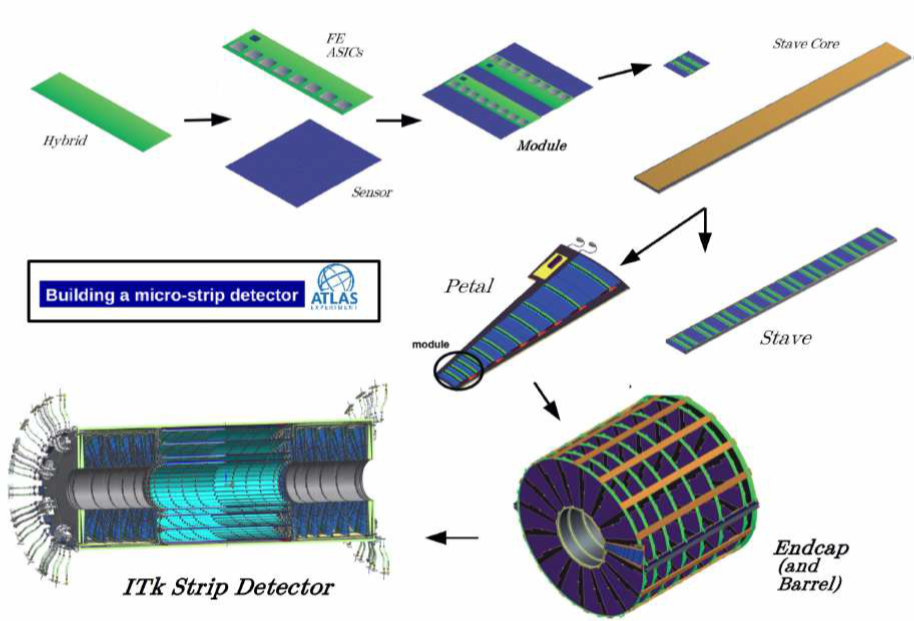
\includegraphics[width=0.75\linewidth]{PictureITKstrip.png}
  \caption{The assembly diagram of the ATLAS ITk Strip Detector \cite{8}
}
  \label{fig:ITKdet}
	\end{center}
\end{figure}

For the CFD purpose, the simplified ITK volume for ITK purge volume is represented by the figure \ref{fig2}.

\begin{figure}[!h]
\begin{center}
  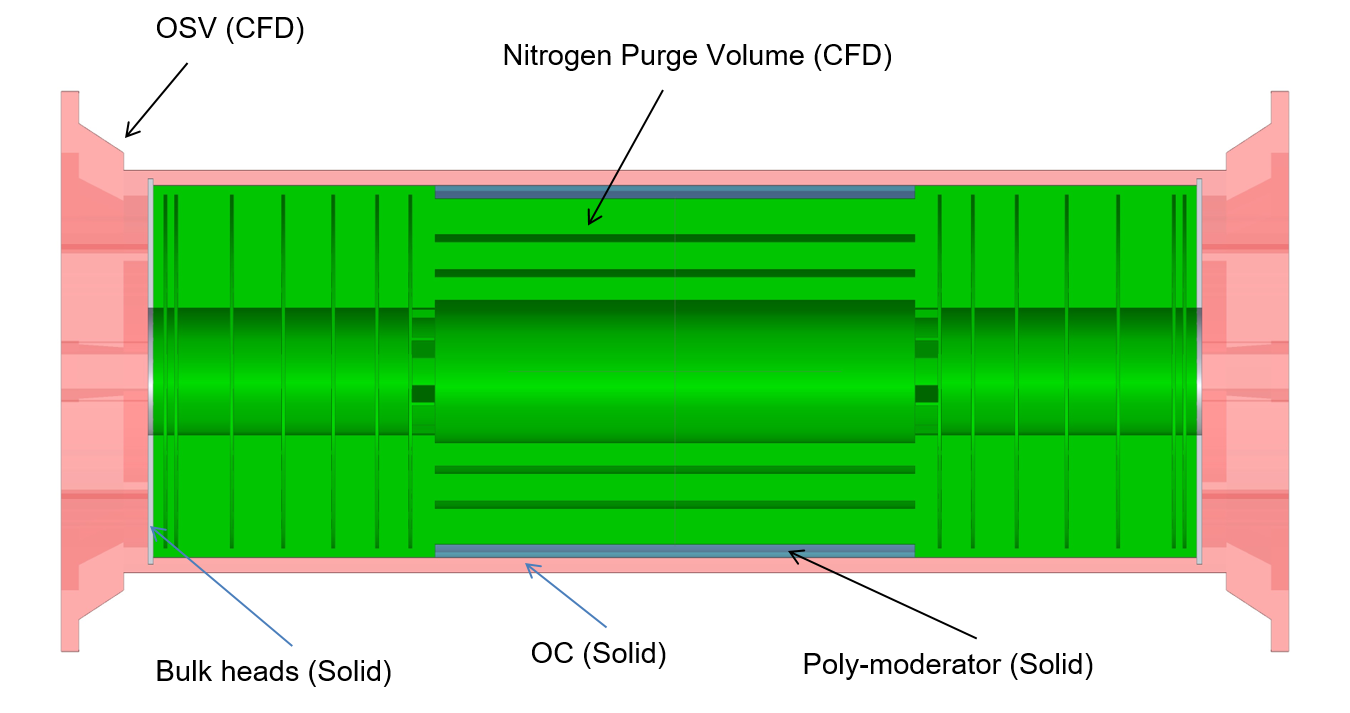
\includegraphics[width=0.60\linewidth]{geometryITK.png}
  \caption{: The ITK - Purge Volume CFD geometry} 
  \label{fig2} 
	\end{center}
\end{figure}


%%%%%%%%%%%%%%%%%%%%%%%%%%%%%%%%%%%%%%%%%%%%%%%%%%

\section{Mathematical (CFD) model}

For the present study, the description of the CFD method with the equations for conservation of mass, momentum,
and species was used. Turbulent flow is assumed for all runs due to high flow rates, leading to the Reynolds averaged
Navier–Stokes equations (RANS), which were then discretized by the finite volume method. The turbulence
model used for enclosed domain was the $k-{\cal E}$ standard approach with standard wall functions. The detailed
equations and background of these balances are mentioned in Ansys Fluent (2019) Users Guide version 19.3, and the
numerical approach is described as follows:

\subsection{Flow field}
The CFD flow solver based on finite volume method is used in the present work to solve Reynolds-averaged
Navier–Stokes (RANS) equations and species transport. The flow is assumed as steady and incompressible. The
conservation equations of continuity and momentum can be represent as follow:
\begin{eqnarray}
\label{eq1}
	\frac{\partial }{\partial t}(\rho )+ \nabla \cdot (\rho \mbox{U})&=&0\\
	\label{eq2}
	\frac{\partial }{\partial t}(\rho \mbox{U})+\nabla \cdot (\rho \mbox{U}\mbox{U})&=&-\nabla p+\nabla \cdot [\mu_t(\nabla \mbox{U} +\nabla \mbox{U}^{\mbox{T}})],
\end{eqnarray}
where the turbulent viscosity is defined as:
\begin{equation}
\label{eq3}
\mu_t=\rho  C_{\mu} \frac{k^2}{{\cal E}}
\end{equation}
The standard $k-{\cal E}$ model was used in the present CFD work. The transport equations for the turbulent
kinetic energy equation and the dissipation rate equation respectively are represent as follow:
\begin{eqnarray} 
\label{eq4}
-\nabla \cdot \left[ \left(\eta + \rho\frac{C_\mu k^2}{\sigma_k {\cal E}}\right)\nabla k \right]+\rho \mbox{U}\cdot\nabla k
&=&\rho C_\mu \frac{k^2}{{\cal E}}(\nabla \mbox{U}+\nabla \mbox{U}^{\mbox{T}})^2 - \rho\\
-\nabla \cdot \left[ \left(\eta + \rho\frac{C_\mu k^2}{\sigma_k {\cal E}}\right)\nabla {\cal E} \right]+\rho \mbox{U}\cdot\nabla {\cal E} &=& \rho C_{{\cal E} 1} C_\mu k (\nabla \mbox{U} +\nabla \mbox{U}^{\mbox{T}})^2 -\rho C_{{\cal E} 2}\frac{k^2}{{\cal E }}
\end{eqnarray}
In addition, the mixing and transport of chemical species can be modeled by solving conservation
equations describing convection, diffusion, and reaction sources for each component species. The general form is given by: 

\begin{equation}
 \frac{\partial }{\partial t}(\rho Y_i)+\nabla \cdot(\rho \mbox{U} Y_i)=-\nabla\cdot\vec{J_i}+R_i +S_i,
\end{equation}
where $Y_i$, the local mass fraction of each species, $R_i$ is the net rate of production of species i by chemical reaction and $S_i$ is the rate of creation by addition from the dispersed phase plus any user-defined sources, $J_i$ is the diffusion flux of species $i$, which arises due to concentration gradients.
\begin{equation}
\vec{J_i}=\left(\rho D_{i,m} + \frac{\mu_t}{S_{C_t}}\right)\nabla Y_i,
\end{equation}
where $D_{i,m}$ is the diffusion coefficient for species, $i$, in the
mixture, and $S_{c_t}$ is the turbulent Schmidt number which
defined as:

\begin{equation}
S_{c_t}=\frac{\mu_t}{\rho D_t},
\end{equation}
where $\mu_t$ is the turbulent viscosity and $D_t$ is the turbulent
diffusivity.

\subsection{CFD geometry}

For the CFD purpose, we started with the simplified ITK volume represented in Figure \ref{fig:3}. 
This geometry does not include the strips volume. As the thermal CFD simulations of the strips volume has priority. 
Therefore, necessity of the new flushing scheme. This should include the nitrogen (N2) Inlets for full distribution via distributed manifold that distributes N2 between the stiffener disk and the detectors. The modified geometry in displayed in Figure \ref{fig:4}. From this new scheme, we introduce the leak points as showed in the modified
ITK geometry in Figure \ref{fig:5}. 

\begin{figure}[!ht]
\begin{center}
  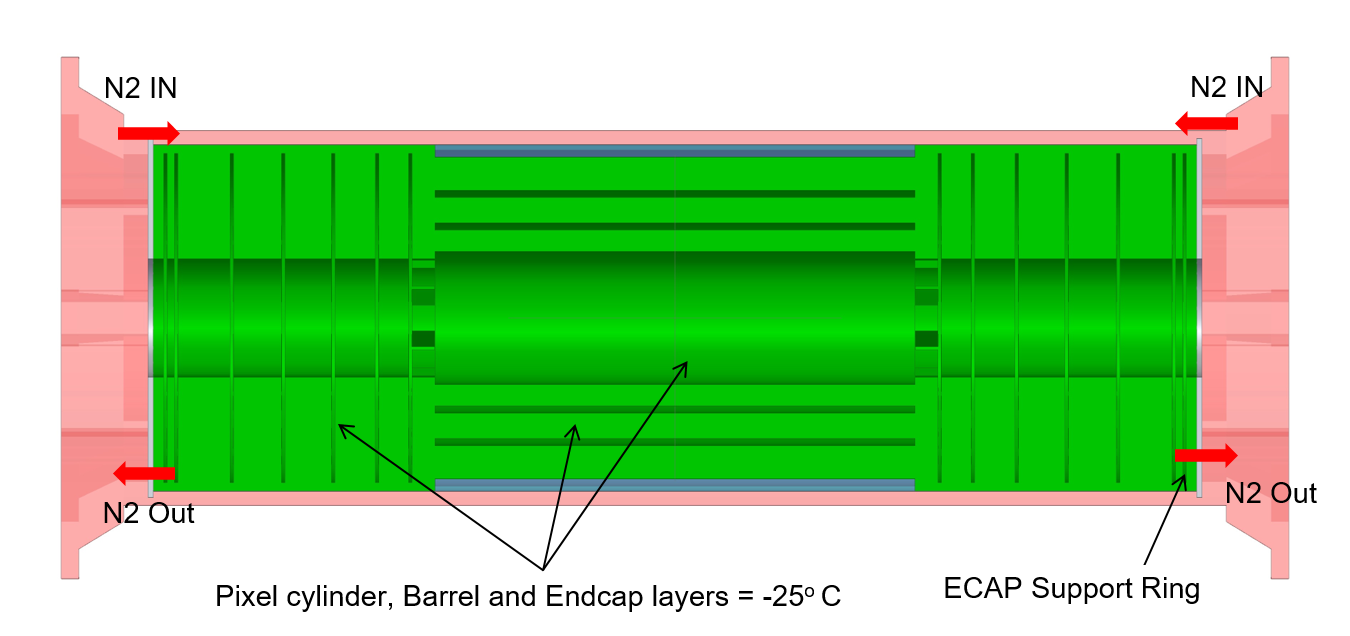
\includegraphics[width=0.50\linewidth]{SR1Case1.png}
  \caption{The N2 gas flushing concepts without the strips. } 
  \label{fig:3} 
	\end{center}
\end{figure}

\begin{figure}[!ht]
\begin{center}
  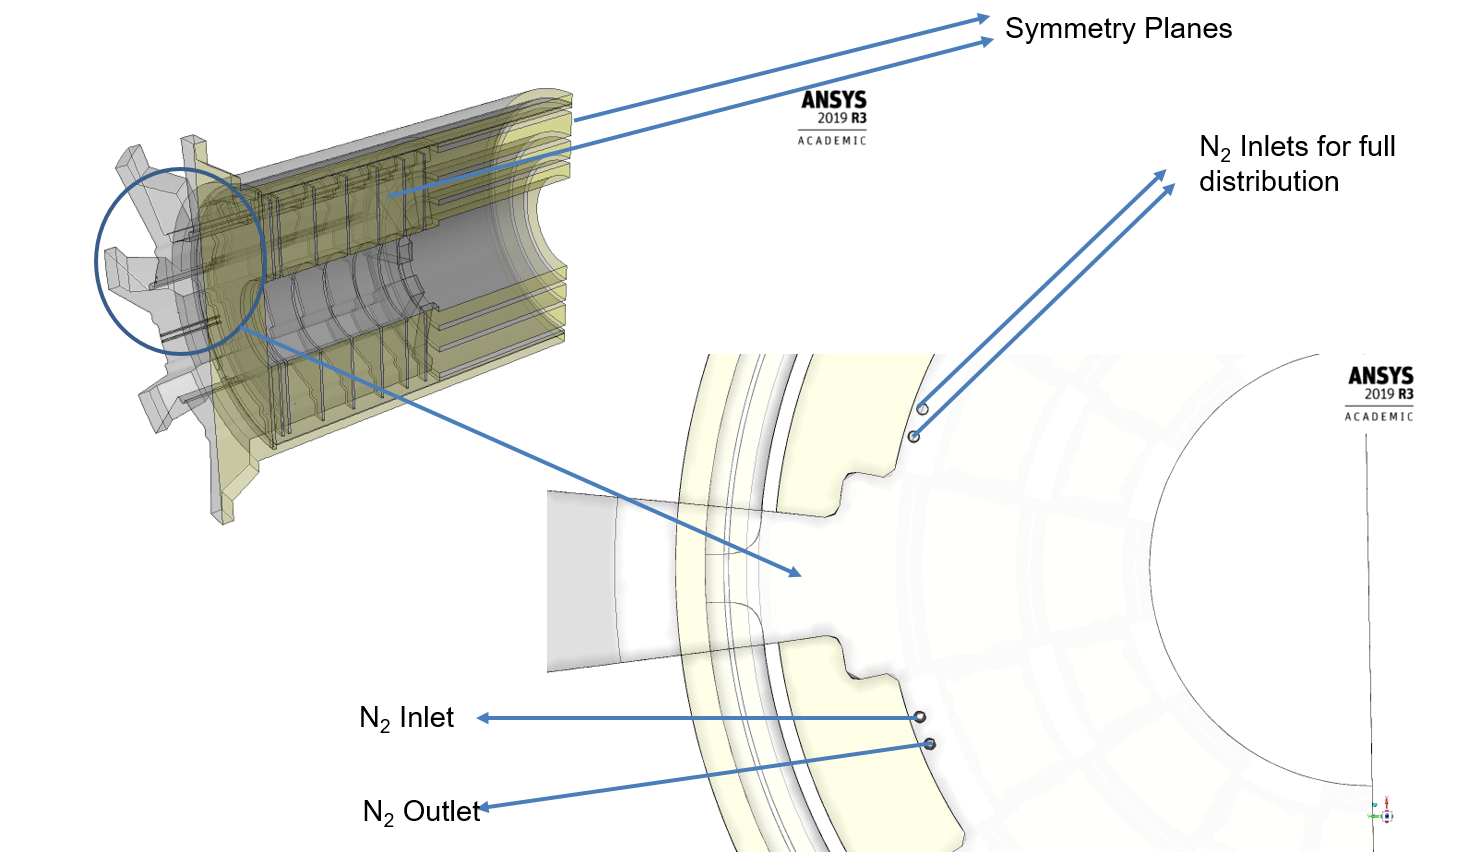
\includegraphics[width=0.50\linewidth]{N2newscheme.png}
  \caption{The N2 gas flushing concepts (modified) with the strips.} 
  \label{fig:4} 
	\end{center}
\end{figure}

\begin{figure}[!ht]
\begin{center}
  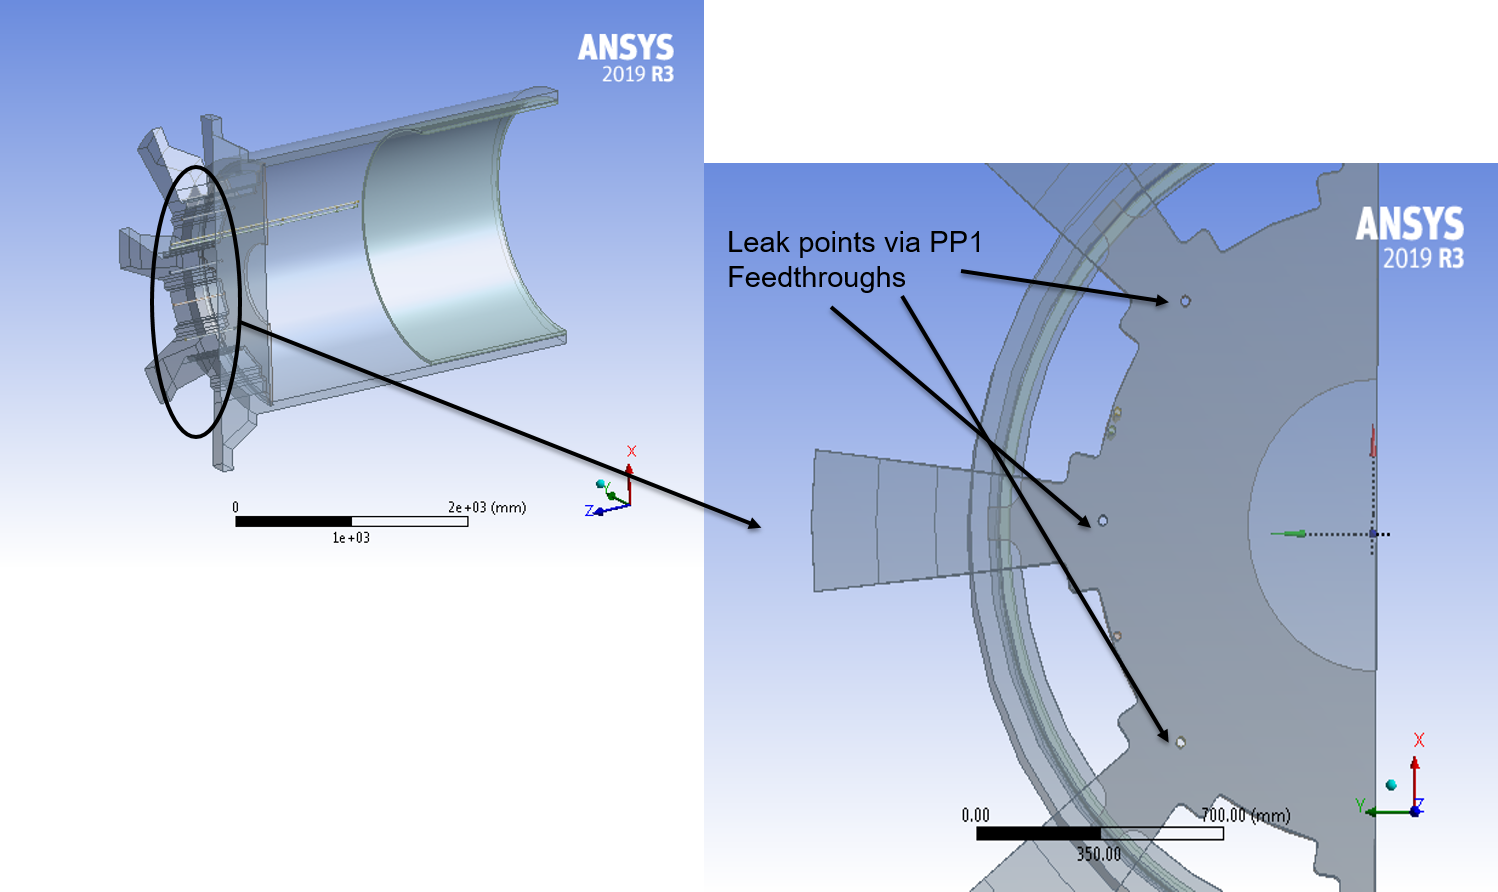
\includegraphics[width=0.50\linewidth]{Picture12.png}
  \caption{ Leak points as showed in the modified ITK geometry. 
}
  \label{fig:5}
\end{center}
\end{figure}
%%%%%%%%%%%%%%%%%%%%%%%%%%%%%%%%%%%%%%%%%%%%%%%%%%%%%%%%%%%%%%%%

\subsection{The model settings and boundary conditions}

In order to solve the system of equations proposed above, it is necessary to delimit the solution domain.
We introduced Leaks via PP1 feed through at a leak rate of 0.1 \mbox{L/s} air of the room temperature introduce near bulkhead. The total rate of 0.1 \mbox{l/s} should be divided over 12 leak points as showed in the modified ITK geometry and the N2 being pump at the velocity of 2.4 \mbox{m/s}. We use air humid with three species: nitrogen (mass fraction of 0.78), oxygen (mass fraction of 0.21), vapour of water (mass fraction of 0.01).
The summary of  model settings and boundary conditions is listed in Table \ref{tab:eventselection}. 
The simulation is run for two cases, first SR1 without leaks and SR1 with leaks. results are presented in section \ref{result}


\begin{table}[!ht]
  \vspace{-10pt}
  \caption{\footnotesize{The Model settings and boundary conditions of CFD simulation.}}
  \begin{center}
    \begin{footnotesize}
     \scalebox{0.8}{     $\mbox{ }$
      \begin{tabular}{l|>{\arraybackslash}p{0.7\linewidth}}
          \hline
          \textbf{Classification} & Settings  \\
          \hline
          \textsc{Solver}& - Fluent solver, $3-D$ simulation\\
          & - Unsteady state analysis (second order explicit)\\
        \textsc{Energy equation}  & - Activated \\
       \textsc{Viscous model}   & - Realizable $k-{\cal E}$ model\\
          & - Standards wall functions \\
					 & - Full buoyancy effects \\
				 \textsc{Species model} & - Species transport \\
				& - Mixture properties \\
				& - Eddy dissipation \\
				& - Species transport \\
				& - Option diffusion, Energy Source \\
          \hline
        \textsc{Boundary conditions} & Physical parameters\\
        \hline
        \textsc{Leak inlets} & - Mass flow rate: 0.1/12 kg/s \\
          & - Mass fraction: Nitrogen (0.78)\\
          & - Mass fraction: Oxygen (0.21)  \\
          & - Mass fraction: Water vapour (0.01) \\
					&- Temperature: 0$^{\circ}$  C\\
					&- dew point: -30$^{\circ}$  C\\
          \textsc{Inlets} &- Velocity: 2.4 m/s\\
					         &- pressure: 1 mbar\\
&- Temperature: 15$^{\circ}$  C\\
& - Mass fraction: Nitrogen (1.0) \\
   \textsc{Outlet} &  - Gauge pressure: 4 mbar\\
	& - Temperature: 15$^{\circ}$ C \\
	 \textsc{Skin material}& - k = 50 W/mK\\
        \hline
        \end{tabular}
    }
  \vspace{-30pt}
  \end{footnotesize}
  \end{center}
     \vspace{-10pt}
  \vspace{-10pt}
  \label{tab:eventselection}
%\end{sidewaystable}
\end{table}


\subsection{Model results\label{result}}
The results of the simulation for both cases (SR1 without leaks and  SR1 with leaks). The SR1 without leaks results are display in Figures \ref{fig:6}, \ref{fig:7} and \ref{fig:8}. while the SR1 with leaks results are display in Figures \ref{fig:9}, \ref{fig:10} and \ref{fig:11}. 
The most important parameters such: Temperature, velocity and relative humidity are presented.
\begin{figure}[!h]
\centering
  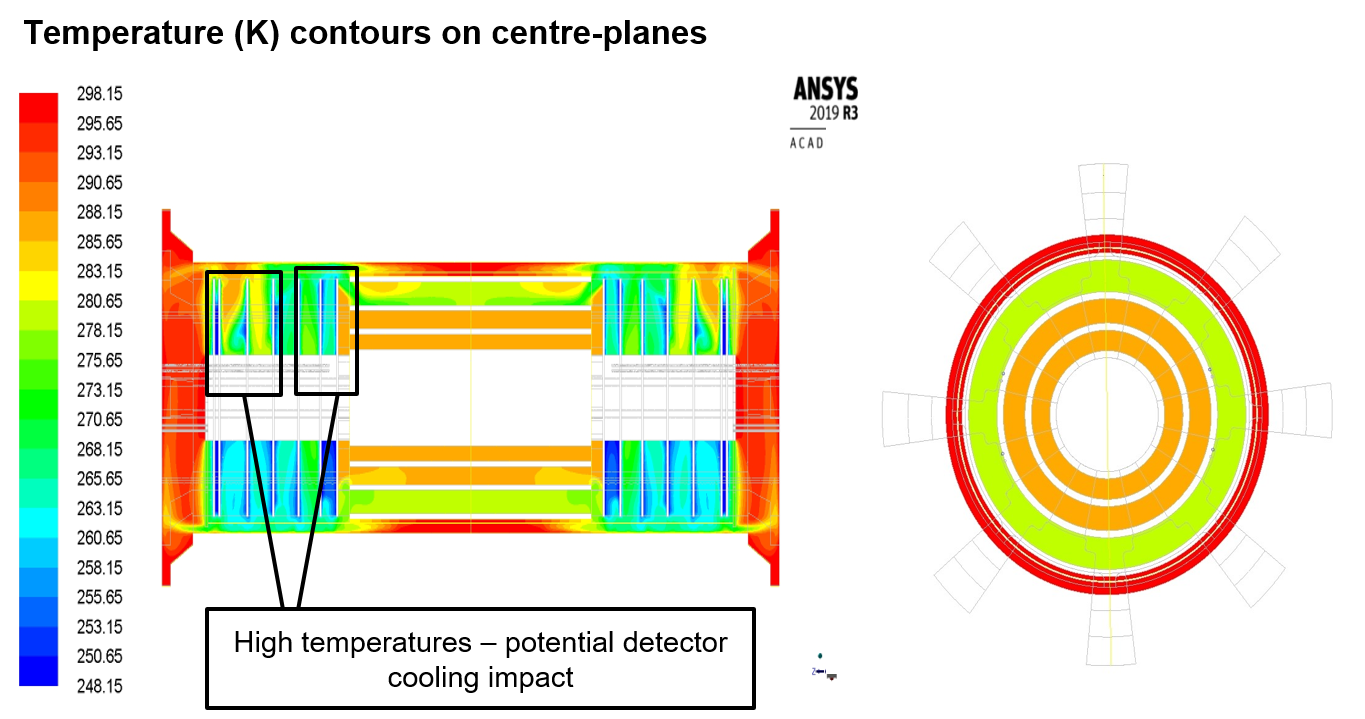
\includegraphics[width=0.60\linewidth]{Picture20.png}
  \caption{Temperature (K) contours on centre-plane for SR1 without leaks 
}
  \label{fig:6}
\end{figure}

\begin{figure}[!h]
\begin{center}
  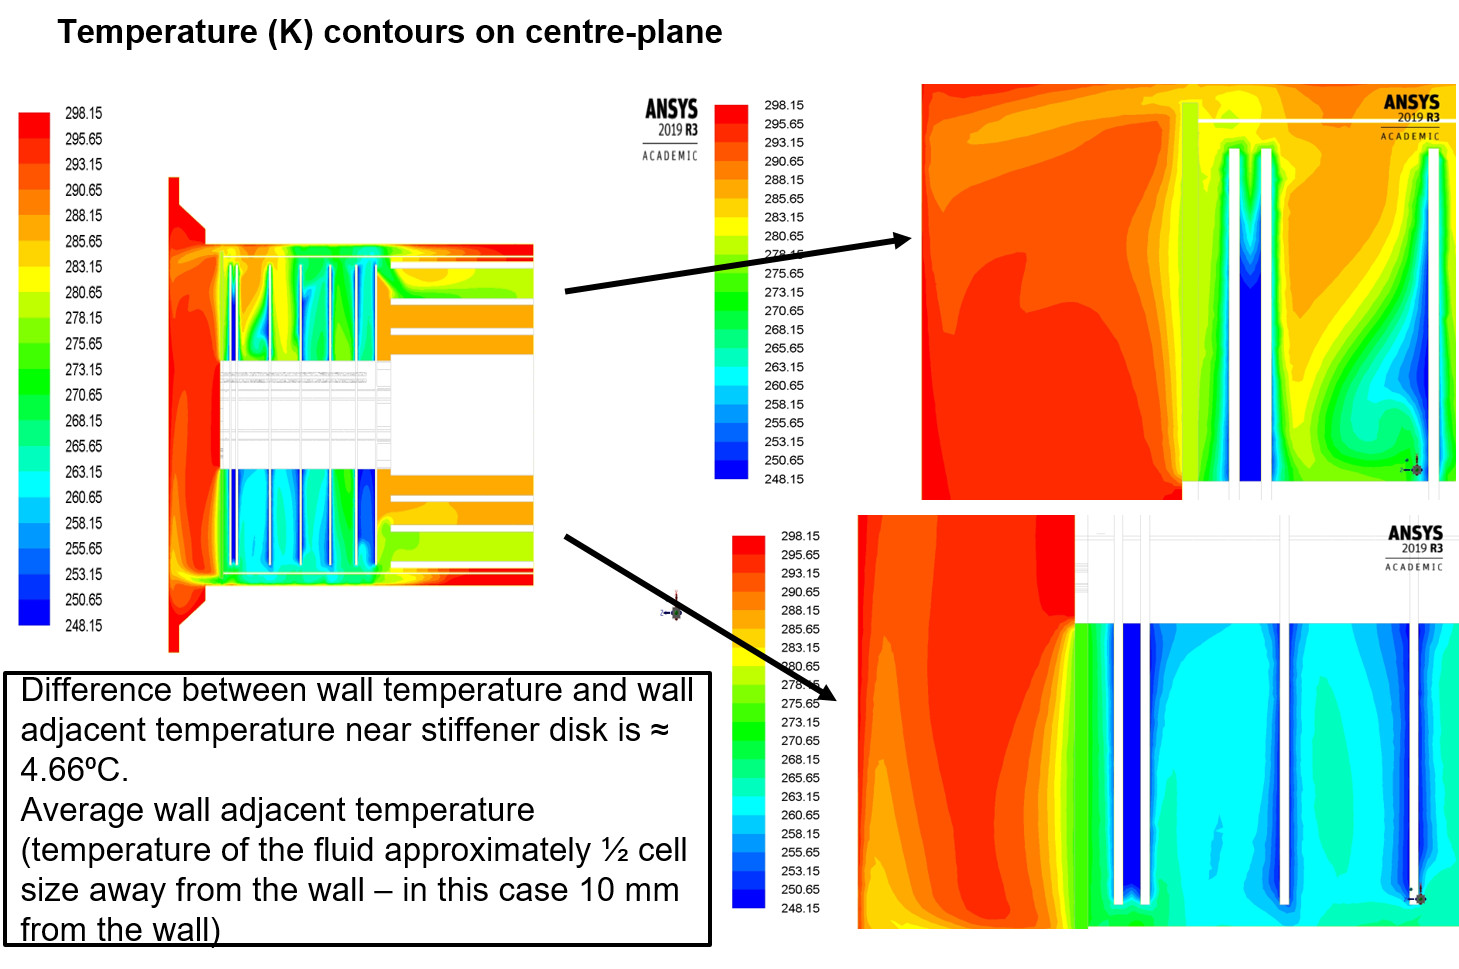
\includegraphics[width=0.60\linewidth]{Picture22.png}
  \caption{Temperature (K) contours on centre-plane for SR1 without leaks 
with zoom in the box regions }
  \label{fig:7}
	\end{center}
\end{figure}

\begin{figure}[!h]
\begin{center}
  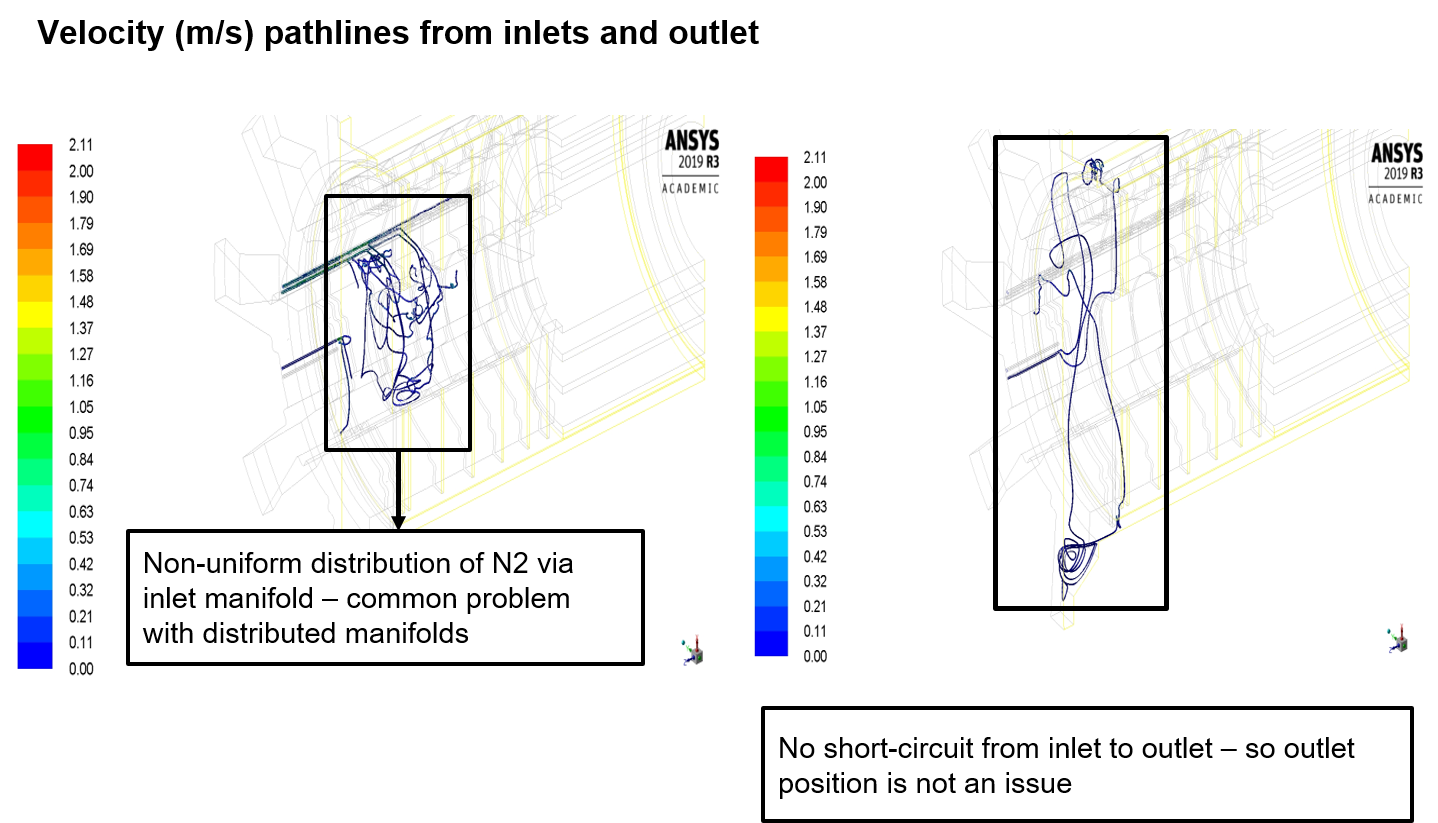
\includegraphics[width=0.80\linewidth]{Picture23.png}
  \caption{ Velocity (m/s) pathlines from inlets and outlet for SR1 without leaks }
  \label{fig:8}
	\end{center}
\end{figure}


\begin{figure}[!h]
\begin{center}
  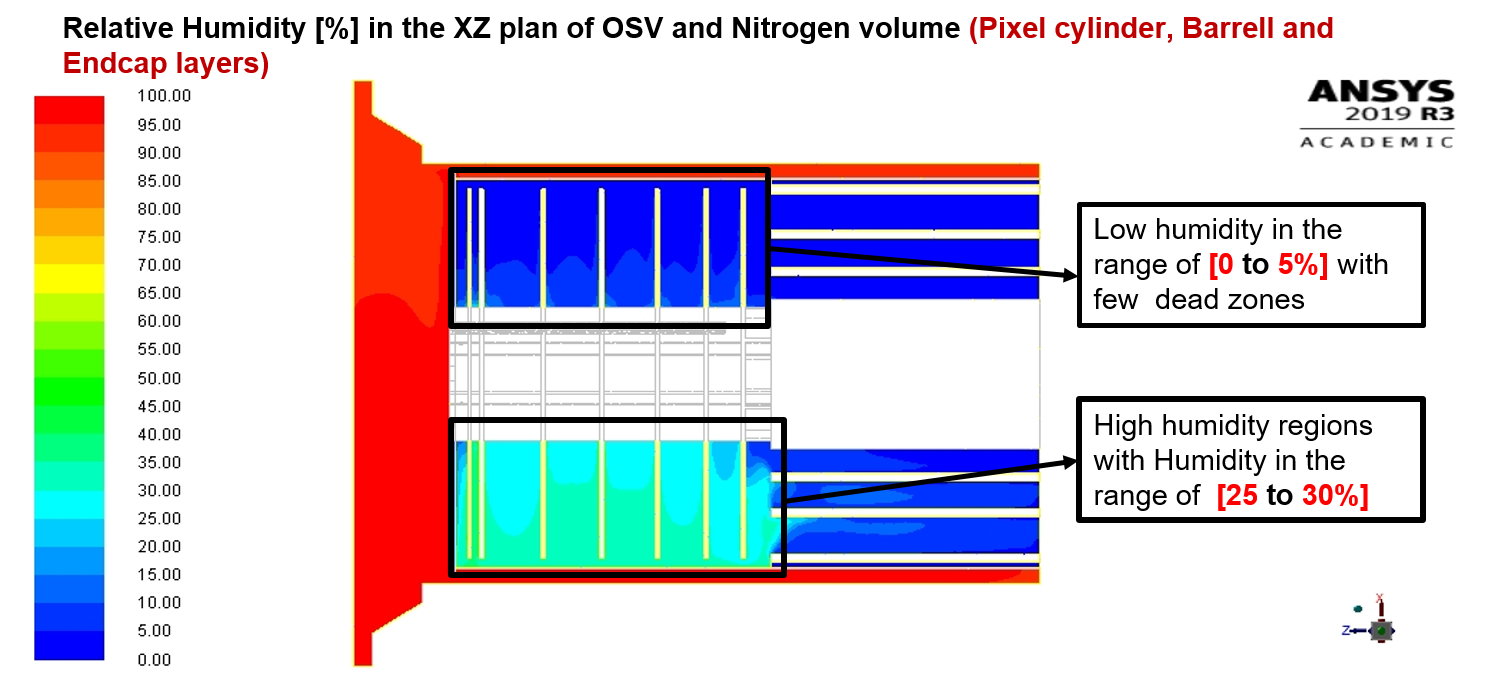
\includegraphics[width=0.69\linewidth]{Picture16.png}
  \caption{Humidity in ITK (Pixel cylinder, Barrell and Endcap layers) for SR1 with leaks }
  \label{fig:9}
	\end{center}
\end{figure}
\begin{figure}[!h]
\begin{center}
  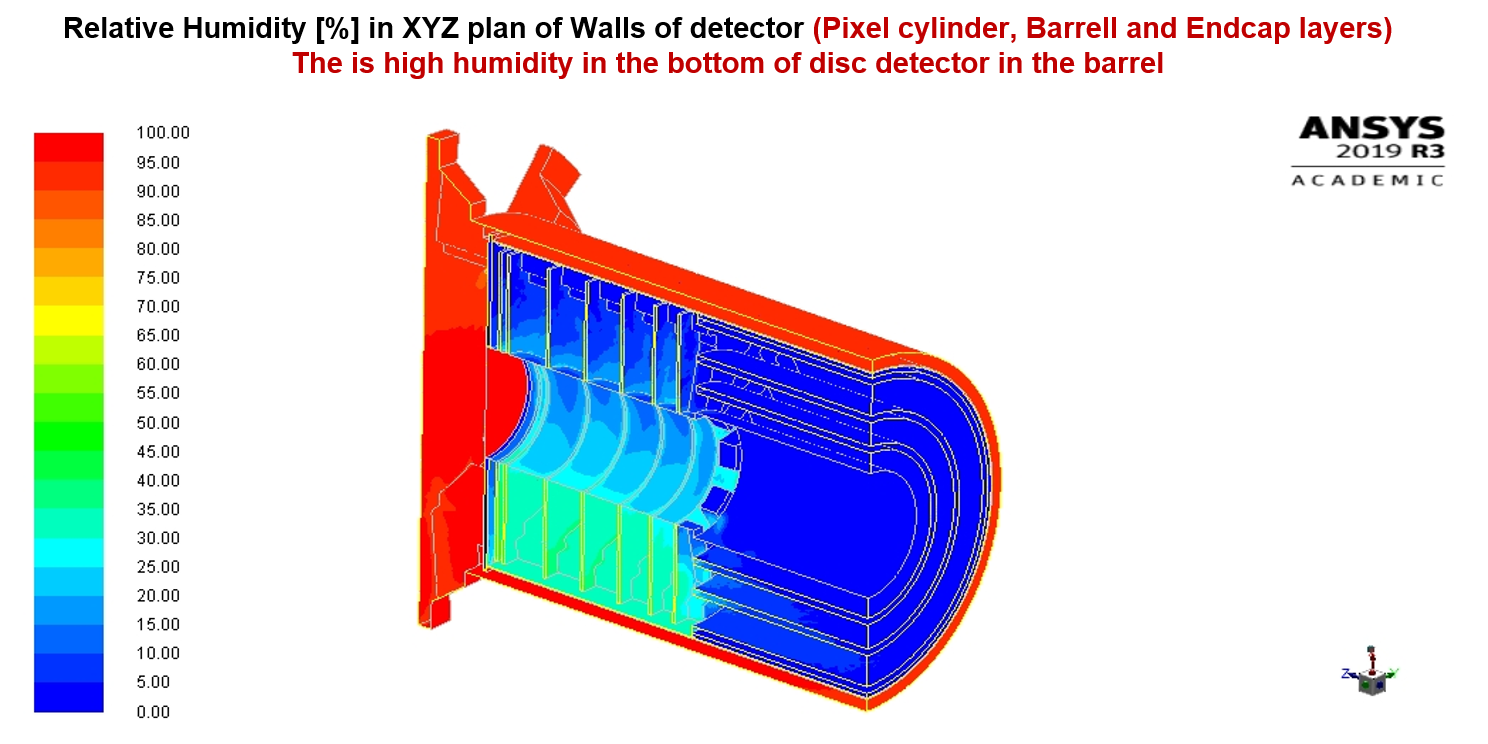
\includegraphics[width=0.69\linewidth]{Picture14.png}
  \caption{Relative Humidity in ITK (Pixel cylinder, Barrell and Endcap layers) for SR1 with leaks }
  \label{fig:10}
	\end{center}
\end{figure}

\begin{figure}[!h]
\begin{center}
  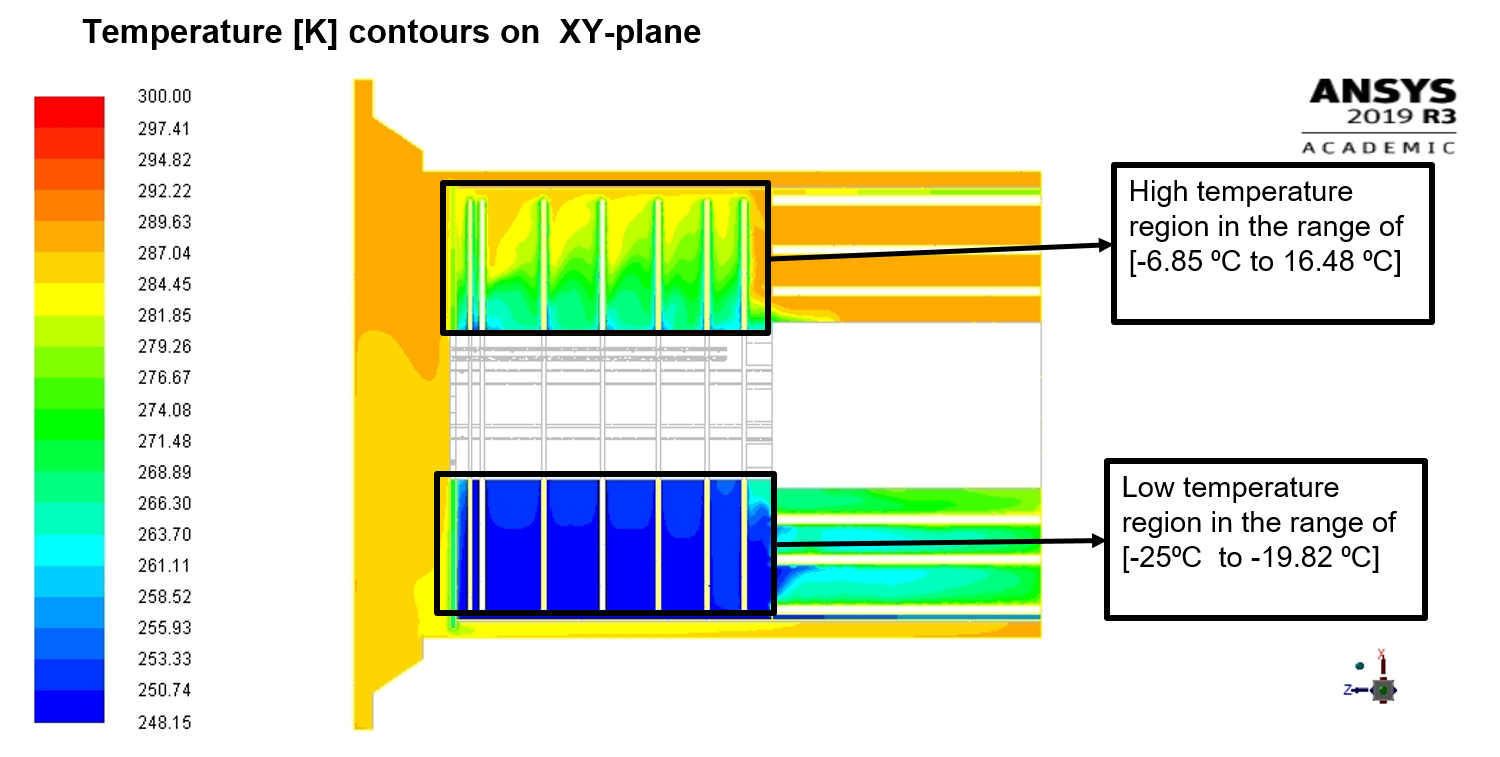
\includegraphics[width=0.69\linewidth]{Picture15.png}
  \caption{Relative humidity in XY plan of the ITK (Pixel cylinder, Barrell and Endcap layers) for SR1 with leaks }
  \label{fig:11}
	\end{center}
\end{figure}

\section{Results and Discussion}


%\section{Results and Discussion}
%
%\begin{figure}
  %\includegraphics[width=0.69\linewidth]{ITKGV.png}
  %\caption{ITK Volume}
  %\label{fig:boat1}
%\end{figure}
%




%Guo, W., Ying, A., Ni,M., & Abdou,M. A. (2006). A numerical
%study of the interactions between viscous flow, transport
%and kinetics in fixed bed reactors. Computers and Chemical
%Engineering, 26(3), 333–357.
%

%\vspace{-10pt}
\section{Acknowlegments}
We thank CERN and all associated staff for the very successful operation of the LHC.
The support of the National Research Foundation (NRF) and Department of Science and Technology, both of South Africa, is acknowledged. Similar acknowledgements apply for all participating institutions in the ATLAS Collaboration. Support from  WLCG is acknowledged.

\clearpage
%\vspace{-10pt}
%\section*{References}
%\bibliographystyle{iopart-num}
%\bibliography{CFDinATLAS}
\begin{thebibliography}{99}
\bibitem{11}  CERN, “Cern public webpages.” Accessed on 22 March 2018 at https://home.
\bibitem{1} ATLAS collaboration, The ATLAS Experiment at the CERN Large Hadron Collider, JINST 3, S08003 (2008).
\bibitem{2} LHC, http://home.web.cern.ch/about/accelerators/large-hadron-collider and CERN, http://home.web.cern.ch; L. Evans and P. Bryant, LHC Machine, JINST 3, S08001 (2008).
\bibitem{3} ATLAS collaboration, Observation of a new particle in the search for the Standard Model Higgs
boson with the ATLAS detector at the LHC, Phys. Lett. B 716, 1 (2012); CMS collaboration, Observation of a new boson at a mass of 125GeV with the CMS experiment at the LHC, Phys. Lett. B 716, 30 (2012).
\bibitem{4} F. Englert and R. Brout, Broken Symmetry and the Mass of Gauge Vector Mesons,
Phys. Rev. Lett. 13, 321 (1964); P.W. Higgs, Broken Symmetries and the Masses of Gauge Bosons, Phys. Rev. Lett. 13 508, (1964).
\bibitem{5} ATLAS collaboration, ATLAS Letter of Intent Phase-I Upgrade, CERN-2011-012, LHCC-I-020 (2011).
\bibitem{6} ATLAS collaboration, ATLAS Letter of Intent Phase-II Upgrade, CERN-2012-022, LHCC-I-023 (2012).
\bibitem{7} Marco Oriunno, SLAC, ITK Volume Purge CFD  (ITK week Jan 2019)
\bibitem{8} The ATLAS Collaboration., Technical Design Report for the ATLAS Inner Tracker Strip Detector
               Reference: CERN-LHCC-2017-005 ATLAS-TDR-025. CERN, September 16, 2016. cern/.
\end{thebibliography}
\end{document}

